%%%%%%%%%%%%%%%%%%%%%%%%%%%%%%%%%%%%%%%%%
% -- TACTICAL COMPUTING LABORATORIES
% -- LATEX TEMPLATE
%%%%%%%%%%%%%%%%%%%%%%%%%%%%%%%%%%%%%%%%%

%----------------------------------------------------------------------------------------
%	PACKAGES AND DOCUMENT CONFIGURATIONS
%----------------------------------------------------------------------------------------

\documentclass{article}

\usepackage[margin=1.0in]{geometry}
\usepackage[version=3]{mhchem} % Package for chemical equation typesetting
\usepackage{siunitx} % Provides the \SI{}{} and \si{} command for typesetting SI units
\usepackage{graphicx} % Required for the inclusion of images
%\usepackage{natbib} % Required to change bibliography style to APA
\usepackage{amsmath} % Required for some math elements 
\usepackage[utf8]{inputenc}
\usepackage[english]{babel}
\usepackage[parfill]{parskip}
\usepackage{array}
\usepackage{algorithm}
\usepackage{algcompatible}
\usepackage{listings}
\usepackage{xcolor}
\usepackage{courier} % for \texttt{}
\usepackage{dirtree}
\usepackage{pgfgantt}
\usepackage{multirow}
\usepackage{xargs}
\usepackage{xcolor}
\usepackage[colorinlistoftodos,prependcaption,textsize=tiny]{todonotes}
\newcommandx{\unsure}[2][1=]{\todo[linecolor=red,backgroundcolor=red!25,bordercolor=red,#1]{#2}}
\newcommandx{\change}[2][1=]{\todo[linecolor=blue,backgroundcolor=blue!25,bordercolor=blue,#1]{#2}}
\newcommandx{\info}[2][1=]{\todo[linecolor=OliveGreen,backgroundcolor=OliveGreen!25,bordercolor=OliveGreen,#1]{#2}}
\newcommandx{\improvement}[2][1=]{\todo[linecolor=Plum,backgroundcolor=Plum!25,bordercolor=Plum,#1]{#2}}
\newcommandx{\thiswillnotshow}[2][1=]{\todo[disable,#1]{#2}}
\newcommand\mynote[1]{\textcolor{red}{#1}}

\RequirePackage{epstopdf}
\RequirePackage{tabularx}
\RequirePackage{xstring}
\RequirePackage{hyperref}
\RequirePackage{fancyhdr}

%-- setup paragraphs and margins
\setlength{\parindent}{1em}
\setlength{\parskip}{1em}

%-- code listing setup
\lstdefinestyle{base}{
  language=C++,
  numbers=left,
  stepnumber=1,
  emptylines=1,
  breaklines=true,
  basicstyle=\ttfamily\color{black},
  moredelim=**[is][\color{red}]{@}{@},
}

%-- setup hyperlinks
\hypersetup{
  colorlinks=true,
  linktoc=all,
  linkcolor=black,
  citecolor=black,
  urlcolor=black
}
%--

\setlength\parindent{0pt} % Removes all indentation from paragraphs

\renewcommand{\labelenumi}{\alph{enumi}.} % Make numbering in the enumerate environment by letter rather than number (e.g. section 6)

%\usepackage{times} % Uncomment to use the Times New Roman font
%----------------------------------------------------------------------------------------
%	DOCUMENT LAYOUT INFORMATION
%----------------------------------------------------------------------------------------
\pagestyle{fancy}
\lhead{}
\chead{CircusTent}
\rhead{}
\lfoot{Version 1.0} %-- format: TR YYYY-RRR-V.V; y = year; r = report; v = version
\cfoot{CircusTent}
\rfoot{\thepage}      % -- page number

%----------------------------------------------------------------------------------------
%	DOCUMENT INFORMATION
%----------------------------------------------------------------------------------------

\title{CircusTent Developer Guide} % Title

\author{Tactical Computing Laboratories, LLC} % Author name

\date{} % Date for the report

\begin{document}

%-- begin TCL logo
\begin{figure}
\begin{center}

\includegraphics[width=2in]{figures/circus_tent.png} % Include the logo
\end{center}
\end{figure}
%-- end TCL logo

\maketitle % Insert the title, author and date
\thispagestyle{fancy} %-- force the fancyhdr

\begin{center}
\begin{tabular}{l r}
Date: & November 27, 2019 \\ % Date the experiment was performed
Revision: & 1.0 \\         % revision number
Authors: & John D. Leidel\\ % Author names
& jleidel@tactcomplabs.com\\
\end{tabular}
\end{center}

% If you wish to include an abstract, uncomment the lines below
% \begin{abstract}
% Abstract text
% \end{abstract}

%----------------------------------------------------------------------------------------
%       TOC
%----------------------------------------------------------------------------------------

\clearpage
\tableofcontents
\clearpage

%----------------------------------------------------------------------------------------
%       List of Figures
%----------------------------------------------------------------------------------------

\clearpage
\listoffigures
\lstlistoflistings
\listoftables
%\listofalgorithms
\clearpage

%----------------------------------------------------------------------------------------
%	SECTION 1
%----------------------------------------------------------------------------------------
\clearpage
\section{Introduction}
\label{sec:Introduction}

The CircusTent benchmark infrastructure is constructed in a manner that provides
users the ability to extend the existing set of benchmark implementations (herein 
referred to as \textit{Impls}) with additional programming models.  As we see in Figure~\ref{fig:Arch}, 
the CircusTent infrastructure contains a top-level driver object that is manifested as a 
binary executable.  Within this binary executable, we use a set of driver objects that handle 
the initialization and parsing of various runtime options.  We also use a base implementation 
class that is inherited from all other implementations in order to provide a common implementation 
interface.  

\begin{figure}[h]
\begin{center}
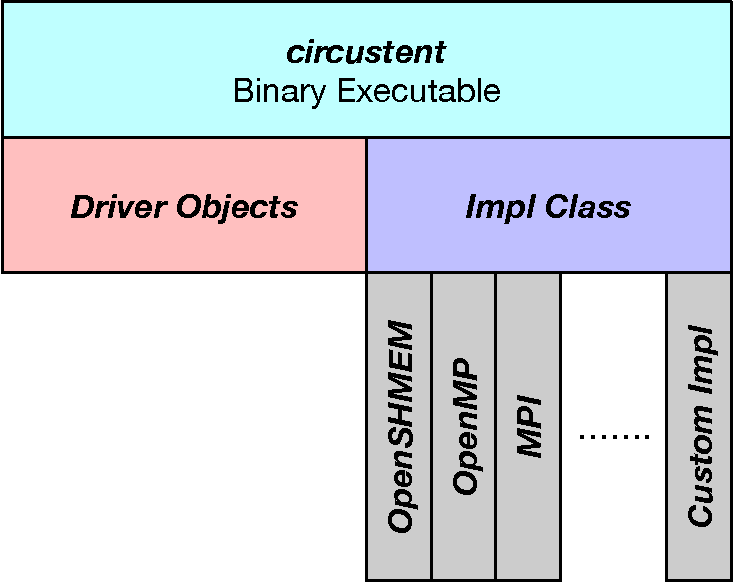
\includegraphics[width=4in]{figures/Arch.pdf}
\vspace*{8pt}
\caption{CircusTent Architecture}
\label{fig:Arch}
\end{center}
\end{figure}

The remainder of this document is organized as follows.  Section~\ref{sec:Building} 
describes the process by which to build CircusTent from source.  Section~\ref{sec:BackendDev} 
describes the process by which to modify the existing portions of the source tree and adding 
the necessary files for new backend implementations.  

%----------------------------------------------------------------------------------------
%	SECTION 2
%----------------------------------------------------------------------------------------
\clearpage
\section{Building CircusTent}
\label{sec:Building}

\subsection{Required Packages}
\label{sec:RequiredPackages}

The following packages are required for developers to build and debug 
new CircusTent backend implementations. 

\begin{itemize}
\item CMake 3.4.3+
\item C/C++ Compiler (GCC and Clang have been tested)
\end{itemize}

Optional packages that may be required include:

\begin{itemize}
\item RPM tools to build platform RPMs
\item Debian package tools (deb) for constructing DEB binary payloads
\item Backend specific libraries, runtimes and tool chains
\item System/platform/API debuggers
\end{itemize}

\subsection{Building From Source}
\label{sec:BuildingFromSource}

Building the CircusTent infrastructure can be performed using the following 
steps.

Clone the CircusTent repository:
\begin{verbatim}
$> git clone https://github.com/tactcomplabs/circustent.git
\end{verbatim}

Setup your build tree:
\begin{verbatim}
$> cd circustent
$> mkdir build
$> cd build
\end{verbatim}

Execute CMake to generate the makefiles (where XXX refers 
to the backend that you wish to enable).
\begin{verbatim}
$> cmake -DENABLE_XXX=ON ../
\end{verbatim}

Execute the build.
\begin{verbatim}
$> make
\end{verbatim}

\clearpage
\subsection{Backend Independent CMake Options}
\label{sec:CMakeOptions}

The following CMake options are supported in the base CircusTent 
implementation.  Each option is utilized as follows: 

\begin{verbatim}
$> cmake -DOPTION=ARGS
\end{verbatim}

\begin{table}[!h]
\renewcommand{\arraystretch}{1.3}
\caption{CMake Build Options}
\label{tab:cmakeoptions}
\centering
\begin{tabular}{c|c|c}
\hline
\textbf{Option} & \textbf{Required Args} & \textbf{Description}\\
\hline
\texttt{CMAKE\_C\_FLAGS} & Compiler Flags & Appends flags to the base CFLAGS\\
\hline
\texttt{CMAKE\_CXX\_FLAGS} & Compiler Flags & Appends flags to the base CXXFLAGS\\
\hline
\texttt{CMAKE\_INSTALL\_PREFIX} & Installation Path & Sets the installation path (\texttt{make install})\\
\hline
\texttt{CIRCUSTENT\_BUILD\_RPM} & ON/OFF & Enables RPM packaging\\
\hline
\texttt{CIRCUSTENT\_BUILD\_DEB} & ON/OFF &  Enables DEB packaging\\
\hline
\texttt{CIRCUSTENT\_BUILD\_TGZ} & ON/OFF & Enables TGZ packaging\\
\hline
\texttt{BUILD\_ALL\_TESTING} & ON/OFF & Enables the test harness (\texttt{make test})\\
\hline
\end{tabular}
\end{table}

%----------------------------------------------------------------------------------------
%	SECTION 3
%----------------------------------------------------------------------------------------
\clearpage
\section{Backend Development}
\label{sec:BackendDev}

\subsection{Development Overview}
\label{sec:DevelopmentOverview}

The process by which a new backend implementation is described below.  However, 
we suggest familiarizing yourself with the source tree, especially those noted in 
Section~\ref{sec:FileStructure}.  

\begin{itemize}
\item \textbf{Create the Source Tree}: Create the source tree for the new implementation 
using the guide described in Section~\ref{sec:FileStructure}.  

\item \textbf{Modify the CMake Infrastructure}: Modify the CMake build infrastructure 
in order to integrate the new implementation infrastructure as described in Section~\ref{sec:CMakeMods}.  

\item \textbf{Implement the Backend Implementation}: Implement the backend infrastructure 
in the directory created in the previous step.  This process is described in Section~\ref{sec:BackendImpl}.  

\item \textbf{Modify the Frontend Driver}:  Modify the frontend driver infrastructure in order to 
integrate the new implementation model.  This process is described in Section~\ref{sec:FrontendMods}.  

\item \textbf{Document the Implementation}: The final stage of the implementation is to document the 
runtime details on how the model is constructed, what algorithms are supported and how the infrastructure 
is executed (runtime details) in the top-level \texttt{README.md} file.   
\end{itemize}

\clearpage
\subsection{File Structure}
\label{sec:FileStructure}

The following file hierarchy describes the files that may be required to be modified 
in order to add a new backend implementation.  Please note that all the files are 
relative to the base CircusTent source tree.  Further, the file hierarchy does not 
depict \textit{all} the files in the source tree, only those that may need to be modified.  
Finally, all the files resident under the \texttt{Impl/CT\_NEWIMPL} directory are considered 
to be new files created for the new implementation.  

\vspace{0.125in}
\dirtree{%
.1 CMakeLists.txt.
.1 LICENSE.
.1 README.md.
.1 include.
.2 CircusTent.
.3 CTBaseImpl.h.
.1 src.
.2 CircusTent.
.3 CMakeLists.txt.
.3 CT\_Main.cpp.
.3 Impl.
.4 CMakeLists.txt.
.4 CT\_NEWIMPL.
.5 CMakeLists.txt.
.5 CT\_NEWIMPL\_IMPL.c.
.5 CT\_NEWIMPL.cpp.
.5 CT\_NEWIMPL.h.
}

\clearpage
\subsection{CMake Modifications}
\label{sec:CMakeMods}

The next step in adding the necessary infrastructure for a new implementation 
is to modify the CMake build scripts.  We use CMake to drive the various platform 
and implementation-specific options.  In this section we will present a very simple 
sample of how one might add the necessary CMake logic to enable new backend implementations.  

The first step in this process is to add an implementation-specific logic block to the 
top-level CMake script \texttt{CMakeLists.txt}.  In the implementation-specific flags section, 
we add a new set of directives enclosed by a conditional statement.  This permits users
to specify \texttt{-DENABLE\_NEWIMPL=ON} on the CMake command line.  As we see 
in Listing~\ref{lis:CMakeLogicBlock}, the logic block appends preprocessor directives 
to each of the C and C++ flags.  This step is required as many of the driver and frontend 
functions present in CircusTent make use of preprocessor macros in order to enable/disable 
specific backend implementations.  Please note how you define these preprocessor macros 
as they will be utilized in further steps.  Here, we utilize \texttt{-D\_ENABLE\_NEWIMPL\_}.  

\vspace{0.125in}
\begin{lstlisting}[frame=single,style=base,caption={CMake Logic Block},captionpos=b,label={lis:CMakeLogicBlock}]
#------------------------------------------------------------------------
#-- IMPLEMENTATION-SPECIFIC FLAGS
#------------------------------------------------------------------------
if (ENABLE_OMP)
  set(CMAKE_C_FLAGS "${CMAKE_C_FLAGS} -fopenmp -D_ENABLE_OMP_")
  set(CMAKE_CXX_FLAGS "${CMAKE_CXX_FLAGS} -fopenmp -D_ENABLE_OMP_")
  set(CMAKE_EXE_LINKER_FLAGS "${CMAKE_EXE_LINKER_FLAGS} -fopenmp")
  message(STATUS "ENABLING OpenMP Implementation")
else()
  message(STATUS "DISABLING OpenMP Implementation")
endif()

if (ENABLE_OPENSHMEM)
  set(CMAKE_C_FLAGS "${CMAKE_C_FLAGS} -D_ENABLE_OPENSHMEM_")
  set(CMAKE_CXX_FLAGS "${CMAKE_CXX_FLAGS} -D_ENABLE_OPENSHMEM_")
  message(STATUS "ENABLING OpenSHMEM Implementation")
else()
  message(STATUS "DISABLING OpenSHMEM Implementation")
endif()

@if (ENABLE_NEWIMPL)
  set(CMAKE_C_FLAGS "${CMAKE_C_FLAGS} -D_ENABLE_NEWIMPL_")
  set(CMAKE_CXX_FLAGS "${CMAKE_CXX_FLAGS} -D_ENABLE_NEWIMPL_")
  message(STATUS "ENABLING NEWIMPL Implementation")
else()
  message(STATUS "DISABLING NEWIMPL Implementation")
endif()
\end{lstlisting}

The second step in initializing the necessary CMake infrastructure is to add 
an object definition to frontend CMake script.  This forces the objects created for the 
respective implementation to be linked to the main frontend object.  For this, 
we need to edit the CMake script at \texttt{src/CircusTent/CMakeLists.txt}.  Note that 
we add a single line (Line 21 of Listing~\ref{lis:CMakeObjBlock}) that forces the 
frontend target executable to link with the necessary objects.  

\clearpage
\vspace{0.125in}
\begin{lstlisting}[frame=single,style=base,caption={CMake Object Block},captionpos=b,label={lis:CMakeObjBlock}]
# src/CircusTent CMakeLists.txt
# Copyright (C) 2017-2019 Tactical Computing Laboratories, LLC
# All Rights Reserved
# contact@tactcomplabs.com
#
# See LICENSE in the top level directory for licensing details
#

add_subdirectory(Impl)

set(CTSrcs
CT_Main.cpp
CTOpts.cpp
)

include_directories(${CT_INCLUDE_PATH})
include_directories(${CT_SRC_PATH}/Impl/CT_OMP)

add_executable(circustent ${CTSrcs} $<TARGET_OBJECTS:CT_OMP_OBJS>
                                    $<TARGET_OBJECTS:CT_SHMEM_OBJS>
@				    $<TARGET_OBJECTS:CT_NEWIMPL_OBJS>)@

if (ENABLE_OPENSHMEM)
  target_link_libraries(circustent oshmem mpi)
endif()

install(TARGETS circustent DESTINATION bin)
\end{lstlisting}

The final step in modifying the necessary CMake scripts is to add a directive 
that permits CMake to discover the new implementation directory.  
In order to do so, we must modify the CMake script at 
\texttt{src/CircusTent/Impl/CMakeLists.txt}.  For this, we add a single line 
to add the respective subdirectory as noted in Listing~\ref{lis:CMakeDirBlock}.  

\vspace{0.125in}
\begin{lstlisting}[frame=single,style=base,caption={CMake Subdirectory Block},captionpos=b,label={lis:CMakeDirBlock}]
# src/Impl CMakeLists.txt
#
# Copyright (C) 2017-2019 Tactical Computing Laboratories, LLC
# All Rights Reserved
# contact@tactcomplabs.com
#

add_subdirectory(CT_OMP)
add_subdirectory(CT_OPENSHMEM)
@add_subdirectory(CT_NEWIMPL)@

# EOF
\end{lstlisting}

\clearpage
\subsection{Backend Implementation}
\label{sec:BackendImpl}

\subsubsection{Implementation Header File}

The first stage in the implementation of a new backend is to create the necessary C++ 
header file.  The header file contains the inherited class definition for the unique implementation.  
The header file must contain the following elements: 

\begin{itemize}
\item Inherited class definition using the \texttt{CTBaseImpl} class.
\item Constructor and destructor routines for the inherited class.
\item Overridden functions for \texttt{Execute}, \texttt{AllocateData} and \texttt{FreeData}.  The arguments to these functions cannot be modified.
\item Any private variables to contain the respective internal state.
\item The function prototypes for each logic implementation function.  In adjacent implementations, these functions are written in
\textit{C} for performance.  As a result, these functions are defined as \textit{extern C} functions.  We will follow the same procedure here.
\end{itemize}

We provide an example header file (\texttt{CT\_NEWIMPL.h}) as follows.  

\vspace{0.125in}
\begin{lstlisting}[frame=single,style=base,caption={Sample Header File},captionpos=b,label={lis:SampleHeaderFile}]
//
// _CT_NEWIMPL_H_
//
// Copyright (C) 2017-2019 Tactical Computing Laboratories, LLC
// All Rights Reserved
// contact@tactcomplabs.com
//
// See LICENSE in the top level directory for licensing details
//

/**
 * \class CT_NEWIMPL
 *
 * \ingroup CircusTent
 *
 * \brief CircusTent Sample Implementation
 *
 */

#ifdef _ENABLE_NEWIMPL_

#ifndef _CT_NEWIMPL_H_
#define _CT_NEWIMPL_H_

#include <cstdlib>
#include <ctime>

#include "CircusTent/CTBaseImpl.h"

// Benchmark Prototypes
extern "C" {
/// RAND AMO ADD Benchmark
void RAND_ADD( uint64_t *ARRAY,
               uint64_t *IDX,
               uint64_t iters,
               uint64_t pes );

/// RAND AMO CAS Benchmark
void RAND_CAS( uint64_t *ARRAY,
               uint64_t *IDX,
               uint64_t iters,
               uint64_t pes );

/// STRIDE1 AMO ADD Benchmark
void STRIDE1_ADD( uint64_t *ARRAY,
                  uint64_t *IDX,
                  uint64_t iters,
                  uint64_t pes );

/// STRIDE1 AMO CAS Benchmark
void STRIDE1_CAS( uint64_t *ARRAY,
                  uint64_t *IDX,
                  uint64_t iters,
                  uint64_t pes );

/// STRIDEN AMO ADD Benchmark
void STRIDEN_ADD( uint64_t *ARRAY,
                  uint64_t *IDX,
                  uint64_t iters,
                  uint64_t pes,
                  uint64_t stride );

/// STRIDEN AMO CAS Benchmark
void STRIDEN_CAS( uint64_t *ARRAY,
                  uint64_t *IDX,
                  uint64_t iters,
                  uint64_t pes,
                  uint64_t stride );

/// PTRCHASE AMO ADD Benchmark
void PTRCHASE_ADD( uint64_t *ARRAY,
                   uint64_t *IDX,
                   uint64_t iters,
                   uint64_t pes );

/// PTRCHASE AMO CAS Benchmark
void PTRCHASE_CAS( uint64_t *ARRAY,
                   uint64_t *IDX,
                   uint64_t iters,
                   uint64_t pes );

/// SG AMO ADD Benchmark
void SG_ADD( uint64_t *ARRAY,
             uint64_t *IDX,
             uint64_t iters,
             uint64_t pes );

/// SG AMO CAS Benchmark
void SG_CAS( uint64_t *ARRAY,
             uint64_t *IDX,
             uint64_t iters,
             uint64_t pes );

/// CENTRAL AMO ADD Benchmark
void CENTRAL_ADD( uint64_t *ARRAY,
                  uint64_t *IDX,
                  uint64_t iters,
                  uint64_t pes );

/// CENTRAL AMO CAS Benchmark
void CENTRAL_CAS( uint64_t *ARRAY,
                  uint64_t *IDX,
                  uint64_t iters,
                  uint64_t pes );

/// SCATTER AMO ADD Benchmark
void SCATTER_ADD( uint64_t *ARRAY,
                  uint64_t *IDX,
                  uint64_t iters,
                  uint64_t pes );

/// SCATTER AMO CAS Benchmark
void SCATTER_CAS( uint64_t *ARRAY,
                  uint64_t *IDX,
                  uint64_t iters,
                  uint64_t pes );

/// GATHER AMO ADD Benchmark
void GATHER_ADD( uint64_t *ARRAY,
                 uint64_t *IDX,
                 uint64_t iters,
                 uint64_t pes );

/// GATHER AMO CAS Benchmark
void GATHER_CAS( uint64_t *ARRAY,
                 uint64_t *IDX,
                 uint64_t iters,
                 uint64_t pes );

}


class CT_NEWIMPL : public CTBaseImpl{
private:
  uint64_t *Array;          ///< CT_NEWIMPL: Data array
  uint64_t *Idx;            ///< CT_NEWIMPL: Index array
  uint64_t memSize;         ///< CT_NEWIMPL: Memory size (in bytes)
  uint64_t pes;             ///< CT_NEWIMPL: Number of processing elements
  uint64_t iters;           ///< CT_NEWIMPL: Number of iterations per thread
  uint64_t elems;           ///< CT_NEWIMPL: Number of u8 elements
  uint64_t stride;          ///< CT_NEWIMPL: Stride in elements

public:
  /// CircusTent OpenMP constructor
  CT_NEWIMPL(CTBaseImpl::CTBenchType B,
         CTBaseImpl::CTAtomType A);

  /// CircusTent OpenMP destructor
  ~CT_NEWIMPL();

  /// CircusTent OpenMP exeuction function
  virtual bool Execute(double &Timing,double &GAMS) override;

  /// CircusTent OpenMP data allocation function
  virtual bool AllocateData( uint64_t memSize,
                             uint64_t pes,
                             uint64_t iters,
                             uint64_t stride ) override;

  /// CircusTent OpenMP data free function
  virtual bool FreeData() override;
};

#endif  // _CT_NEWIMPL_H_
#endif  // _ENABLE_NEWIMPL_

// EOF
\end{lstlisting}

\clearpage
\subsubsection{Implementation Overidden Functions}

The next stage in the implementation process is to generate the constructor routine 
and the three required overridden functions.  Note that the entire implementation 
file (\texttt{CT\_NEWIMPL.cpp}) is encapsulated in preprocessor macros in order to prevent 
compilation when the respective backend implementation is disabled.  

For the \texttt{Execute} function, you must interprets the benchmark type and atomic operation type 
in order to determine which logic function to call.  Also note that each logic function call is encapsulated 
in calls to the base function \texttt{MySecond}.  Further, after executing the respective logic function, a call 
to the \texttt{GAM} function in order to derive the number of billions of atomic operations per second.  Refer to 
the API documentation for the arguments for this function.  

The next two functions that must be implemented are the \texttt{AllocateData} and \texttt{FreeData} functions.  
The former allocates any required memory blocks using the prescribed allocation methods.  The latter frees these 
blocks after execution completes.  Both are called by the frontend driver.  

We see an example implementation sample for these functions in Listing~\ref{lis:ImplOverFunc}.  

\vspace{0.125in}
\begin{lstlisting}[frame=single,style=base,caption={Implementation Overidden Functions},captionpos=b,label={lis:ImplOverFunc}]
//
// _CT_NEWIMPL_CPP_
//
// Copyright (C) 2017-2019 Tactical Computing Laboratories, LLC
// All Rights Reserved
// contact@tactcomplabs.com
//
// See LICENSE in the top level directory for licensing details
//

#include "CT_NEWIMPL.h"

#ifdef _CT_NEWIMPL_H_

CT_NEWIMPL::CT_NEWIMPL(CTBaseImpl::CTBenchType B,
               CTBaseImpl::CTAtomType A) : CTBaseImpl("NEWIMPL",B,A),
                                           Array(nullptr),
                                           Idx(nullptr),
                                           memSize(0),
                                           pes(0),
                                           iters(0),
                                           elems(0),
                                           stride(0) {
}

CT_NEWIMPL::~CT_NEWIMPL(){
}

bool CT_NEWIMPL::Execute(double &Timing, double &GAMS){

  CTBaseImpl::CTBenchType BType   = this->GetBenchType(); // benchmark type
  CTBaseImpl::CTAtomType AType    = this->GetAtomType();  // atomic type
  double StartTime  = 0.; // start time
  double EndTime    = 0.; // end time
  double OPS        = 0.; // billions of operations

  // determine the benchmark type
  if( BType == CT_RAND ){
    switch( AType ){
    case CT_ADD:
      StartTime = this->MySecond();
      RAND_ADD( Array, Idx, iters, pes );
      EndTime   = this->MySecond();
      OPS = this->GAM(1,iters,pes);
      break;
    case CT_CAS:
      StartTime = this->MySecond();
      RAND_CAS( Array, Idx, iters, pes );
      EndTime   = this->MySecond();
      OPS = this->GAM(1,iters,pes);
      break;
    default:
      this->ReportBenchError();
      return false;
      break;
    }
  }else if( BType == CT_STRIDE1 ){
    switch( AType ){
    case CT_ADD:
      StartTime = this->MySecond();
      STRIDE1_ADD( Array, Idx, iters, pes );
      EndTime   = this->MySecond();
      OPS = this->GAM(1,iters,pes);
      break;
    case CT_CAS:
      StartTime = this->MySecond();
      STRIDE1_CAS( Array, Idx, iters, pes );
      EndTime   = this->MySecond();
      OPS = this->GAM(1,iters,pes);
      break;
    default:
      this->ReportBenchError();
      return false;
      break;
    }
  }else if( BType == CT_STRIDEN ){
    switch( AType ){
    case CT_ADD:
      StartTime = this->MySecond();
      STRIDEN_ADD( Array, Idx, iters, pes, stride );
      EndTime   = this->MySecond();
      OPS = this->GAM(1,iters,pes);
      break;
    case CT_CAS:
      StartTime = this->MySecond();
      STRIDEN_CAS( Array, Idx, iters, pes, stride );
      EndTime   = this->MySecond();
      OPS = this->GAM(1,iters,pes);
      break;
    default:
      this->ReportBenchError();
      return false;
      break;
    }
  }else if( BType == CT_PTRCHASE ){
    switch( AType ){
    case CT_ADD:
      StartTime = this->MySecond();
      PTRCHASE_ADD( Array, Idx, iters, pes );
      EndTime   = this->MySecond();
      OPS = this->GAM(1,iters,pes);
      break;
    case CT_CAS:
      StartTime = this->MySecond();
      PTRCHASE_CAS( Array, Idx, iters, pes );
      EndTime   = this->MySecond();
      OPS = this->GAM(1,iters,pes);
      break;
    default:
      this->ReportBenchError();
      return false;
      break;
    }
  }else if( BType == CT_SG ){
    switch( AType ){
    case CT_ADD:
      StartTime = this->MySecond();
      SG_ADD( Array, Idx, iters, pes );
      EndTime   = this->MySecond();
      OPS = this->GAM(4,iters,pes);
      break;
    case CT_CAS:
      StartTime = this->MySecond();
      SG_CAS( Array, Idx, iters, pes );
      EndTime   = this->MySecond();
      OPS = this->GAM(4,iters,pes);
      break;
    default:
      this->ReportBenchError();
      return false;
      break;
    }
  }else if( BType == CT_CENTRAL ){
    switch( AType ){
    case CT_ADD:
      StartTime = this->MySecond();
      CENTRAL_ADD( Array, Idx, iters, pes );
      EndTime   = this->MySecond();
      OPS = this->GAM(1,iters,pes);
      break;
    case CT_CAS:
      StartTime = this->MySecond();
      CENTRAL_CAS( Array, Idx, iters, pes );
      EndTime   = this->MySecond();
      OPS = this->GAM(1,iters,pes);
      break;
    default:
      this->ReportBenchError();
      return false;
      break;
    }
  }else if( BType == CT_SCATTER ){
    switch( AType ){
    case CT_ADD:
      StartTime = this->MySecond();
      SCATTER_ADD( Array, Idx, iters, pes );
      EndTime   = this->MySecond();
      OPS = this->GAM(3,iters,pes);
      break;
    case CT_CAS:
      StartTime = this->MySecond();
      SCATTER_CAS( Array, Idx, iters, pes );
      EndTime   = this->MySecond();
      OPS = this->GAM(3,iters,pes);
      break;
    default:
      this->ReportBenchError();
      return false;
      break;
    }
  }else if( BType == CT_GATHER ){
    switch( AType ){
    case CT_ADD:
      StartTime = this->MySecond();
      GATHER_ADD( Array, Idx, iters, pes );
      EndTime   = this->MySecond();
      OPS = this->GAM(3,iters,pes);
      break;
    case CT_CAS:
      StartTime = this->MySecond();
      GATHER_CAS( Array, Idx, iters, pes );
      EndTime   = this->MySecond();
      OPS = this->GAM(3,iters,pes);
      break;
    default:
      this->ReportBenchError();
      return false;
      break;
    }
  }else{
    this->ReportBenchError();
    return false;
  }

  Timing = this->Runtime(StartTime,EndTime);
  GAMS   = OPS/Timing;

  return true;
}

bool CT_NEWIMPL::AllocateData( uint64_t m,
                           uint64_t p,
                           uint64_t i,
                           uint64_t s){
  // save the data
  memSize = m;
  pes = p;
  iters = i;
  stride = s;

  // allocate all the memory
  if( pes == 0 ){
    std::cout << "CT_NEWIMPL::AllocateData : 'pes' cannot be 0" << std::endl;
    return false;
  }
  if( iters == 0 ){
    std::cout << "CT_NEWIMPL::AllocateData : 'iters' cannot be 0" << std::endl;
    return false;
  }
  if( stride == 0 ){
    std::cout << "CT_NEWIMPL::AllocateData : 'stride' cannot be 0" << std::endl;
    return false;
  }

  // calculate the number of elements
  elems = (memSize/8);

  // test to see whether we'll stride out of bounds
  if( stride > 1 ){
    uint64_t end = (pes * iters * stride)-stride;
    if( end > elems ){
      std::cout << "CT_NEWIMPL::AllocateData : 'Array' is not large enough for pes="
                << pes << "; iters=" << iters << ";stride =" << stride
                << std::endl;
      return false;
    }
  }

Array = (uint64_t *)(malloc( memSize ));
  if( Array == nullptr ){
    std::cout << "CT_NEWIMPL::AllocateData : 'Array' could not be allocated" << std::endl;
    return false;
  }

  Idx = (uint64_t *)(malloc( sizeof(uint64_t) * (pes+1) * iters ));
  if( Idx == nullptr ){
    std::cout << "CT_NEWIMPL::AllocateData : 'Idx' could not be allocated" << std::endl;
    free( Array );
    return false;
  }

  // initiate the random array
  srand(time(NULL));
  if( this->GetBenchType() == CT_PTRCHASE ){
    for( unsigned i=0; i<((pes+1)*iters); i++ ){
      Idx[i] = (uint64_t)(rand()%((pes+1)*iters));
    }
  }else{
    for( unsigned i=0; i<((pes+1)*iters); i++ ){
      Idx[i] = (uint64_t)(rand()%(elems-1));
    }
  }
  for( unsigned i=0; i<elems; i++ ){
    Array[i] = (uint64_t)(rand());
  }

  return true;
}

bool CT_NEWIMPL::FreeData(){
  if( Array ){
    free( Array );
  }
  if( Idx ){
    free( Idx );
  }
  return true;
}

#endif

// EOF
\end{lstlisting}

\clearpage
\subsubsection{Implementation Logic}

The next stage of the implementation is to generate the necessary logic functions 
for each combination of algorithm and atomic operation type.  These functions are not 
required to be implemented in \textit{C}, but we provide a sample template below in Listing~\ref{lis:ImplLogic}.  

\vspace{0.125in}
\begin{lstlisting}[frame=single,style=base,caption={Implementation Logic},captionpos=b,label={lis:ImplLogic}]
/*
 * _CT_NEWIMPL_IMPL_C_
 *
 * Copyright (C) 2017-2019 Tactical Computing Laboratories, LLC
 * All Rights Reserved
 * contact@tactcomplabs.com
 *
 * See LICENSE in the top level directory for licensing details
 */

#include <stdint.h>


/* NEWIMPL Benchmark Implementations
 *
 * Benchmark implementations are in the form:
 *
 * void BENCHTYPE_ATOMTYPE( uint64_t *ARRAY, uint64_t *IDX,
 *                          unsigned long long iters,
 *                          unsigned long long pes )
 *
 */

void RAND_ADD( uint64_t *restrict ARRAY,
               uint64_t *restrict IDX,
               uint64_t iters,
               uint64_t pes ){
  // implementation logic
}
\end{lstlisting}

\clearpage
\subsubsection{Implementation CMake Script}

The final stage of the implementation is to generate a CMake script 
for the respective source content.  The easiest method for doing so 
is to copy an example from an adjacent implementation such as the OpenOMP 
directory.  Within this CMake script, ensure that you create the correct object output 
that will be linked to the CircusTent frontend when enabled (\texttt{CT\_NEWIMPL\_OBJS}).
An example CMake script is provided in Listing~\ref{lis:ImplCMakeScript}.    

\vspace{0.125in}
\begin{lstlisting}[frame=single,style=base,caption={Implementation CMake Script},captionpos=b,label={lis:ImplCMakeScript}]
# src/Impl/CT_NEWIMPL CMakeLists.txt
# Copyright (C) 2017-2019 Tactical Computing Laboratories, LLC
# All Rights Reserved
# contact@tactcomplabs.com
#
# See LICENSE in the top level directory for licensing details
#

set(CTNEWIMPLSrcs
)

if (ENABLE_NEWIMPL)
  set(CTNEWIMPLSrcs ${CTNEWIMPLSrcs} CT_NEWIMPL.h CT_NEWIMPL.cpp CT_NEWIMPL_IMPL.c)
  set(CMAKE_C_FLAGS "${CMAKE_C_FLAGS} -std=c99")
endif()

include_directories(${CT_INCLUDE_PATH})
include_directories(./)

add_library(CT_NEWIMPL_OBJS OBJECT ${CTNEWIMPLSrcs})
\end{lstlisting}

\clearpage
\subsection{Frontend Modifications}
\label{sec:FrontendMods}

The final step in adding a new backend implementation is to add the necessary 
driver function in the top-level main program driver.  This file is located 
at \texttt{src/CircusTent/CT\_Main.cpp}.  The first step in doing so is the add
the necessary headers that permit the frontend to access the new class object 
that defines the new implementation.  We enclose this header if the preprocessor 
definition that was utilized in Section~\ref{sec:CMakeMods}.  This enables us to build 
the frontend with or without specific library dependencies.  An example of completing 
the step is show in Listing~\ref{lis:FrontendHeaderMods}.  

\vspace{0.125in}
\begin{lstlisting}[frame=single,style=base,caption={Frontend Header Modifications},captionpos=b,label={lis:FrontendHeaderMods}]
//
// _CT_Main_cpp_
//
// Copyright (C) 2017-2019 Tactical Computing Laboratories, LLC
// All Rights Reserved
// contact@tactcomplabs.com
//
// See LICENSE in the top level directory for licensing details
//

#include "CircusTent/CircusTent.h"
#ifdef _ENABLE_OMP_
#include "Impl/CT_OMP/CT_OMP.h"
#endif
#ifdef _ENABLE_OPENSHMEM_
#include <mpp/shmem.h>
#include "Impl/CT_OPENSHMEM/CT_SHMEM.h"
#endif
@#ifdef _ENABLE_NEWIMPL_
#include "Impl/CT_NEWIMPL/CT_NEWIMPL.h"
#endif@
\end{lstlisting}

The next step in modifying the frontend is to add a driver function 
for the new implementation.  The new driver function will be implemented 
similar to the adjacent OpenMP, OpenSHMEM and MPI drivers.  Use these 
driver functions as a guide.  Also note that the new driver function is required 
to be encapsulated in the same preprocessor statements as noted above.    
Each driver function must call perform the following functions in order:

\begin{itemize}
\item Allocate a new implementation object
\item Call the object's \texttt{AllocateData} function
\item Call the object's \texttt{Execute} function
\item Call the object's \texttt{FreeData} function
\item Call the frontend's \texttt{PrintTiming} function
\item Destroy the object
\end{itemize}

An example driver function is shown in Listing~\ref{lis:FrontendDriverFunc}.  

\clearpage
\vspace{0.125in}
\begin{lstlisting}[frame=single,style=base,caption={Frontend Driver Function},captionpos=b,label={lis:FrontendDriverFunc}]
#ifdef _ENABLE_NEWIMPL_
void RunBenchNEWIMPL( CTOpts *Opts ){
  // init the  object
  CT_NEWIMPL *CT = new CT_NEWIMPL(Opts->GetBenchType(),
                          	Opts->GetAtomType());
  if( !CT ){
    std::cout << "ERROR : COULD NOT ALLOCATE OBJECT" << std::endl;
    return ;
  }

  // Allocate the data
  if( !CT->AllocateData( Opts->GetMemSize(),
                       	Opts->GetPEs(),
                         Opts->GetIters(),
                         Opts->GetStride() ) ){
    std::cout << "ERROR : COULD NOT ALLOCATE MEMORY" << std::endl;
    free( CT );
    return ;
  }

  // Execute the benchmark
  double Timing = 0.;
  double GAMS = 0.;
  if( !CT->Execute(Timing,GAMS) ){
    std::cout << "ERROR : COULD NOT EXECUTE BENCHMARK" << std::endl;
    CT->FreeData();
    free( CT );
    return ;
  }

  // Free the data
  if( !CT->FreeData() ){
    std::cout << "ERROR : COULD NOT FREE THE MEMORY" << std::endl;
    free( CT );
    return ;
  }

  // Print the timing
  PrintTiming( Timing, GAMS );

  // Destroy the object
  free(CT);
}
#endif
\end{lstlisting}

The final stage in modifying the frontend is to insert a call to the new 
implementation driver function in the \texttt{main} function.  This call 
must be encapsulated by the same preprocessor macros as mentioned 
above.  An example of doing so is shown in Listing~\ref{lis:FrontendMainFunc}.  

\clearpage
\vspace{0.125in}
\begin{lstlisting}[frame=single,style=base,caption={Frontend Main Modifications},captionpos=b,label={lis:FrontendMainFunc}]
 if( (!Opts->IsHelp()) && (!Opts->IsList()) ){
    // execute the benchmarks
#ifdef _ENABLE_OMP_
    RunBenchOMP(Opts);
#endif
#ifdef _ENABLE_OPENSHMEM_
    RunBenchOpenSHMEM(Opts);
#endif
#ifdef _ENABLE_NEWIMPL_
    RunBenchNEWIMPL(Opts);
#endif
  }
\end{lstlisting}

%----------------------------------------------------------------------------------------
%	BIBLIOGRAPHY
%----------------------------------------------------------------------------------------

\clearpage
%\bibliography{refs.bib}
%\bibliographystyle{IEEEtran}


%----------------------------------------------------------------------------------------


\end{document}
